\chapter{Definizione del Problema}
\label{cap:definizione}

In questo capitolo viene presentata la definizione del problema affrontato nella tesi, con l'obiettivo di chiarire il contesto, gli attori coinvolti e i vincoli che caratterizzano il sistema. Dopo una prima descrizione generale dello scenario applicativo, verranno introdotte le principali assunzioni adottate, seguite dalla formalizzazione dei concetti base, dalla formulazione del problema e dalle proprietà che il sistema garantisce.

% ------------------------------------------------------------ %

\section{Scenario e Architettura di Riferimento}
\label{sec:scenario_applicativo}

Il sistema oggetto di questa tesi affronta il problema della distribuzione e schedulazione di task computazionali in un insieme di nodi di un cluster distribuito, nel rispetto di un insieme di politiche volte a governare le proprietà dei nodi di esecuzione, la gestione dei dati necessari all'elaborazione e i vincoli associati ai task stessi.

Un insieme di utenti esterni sottomette richieste di esecuzione di task al sistema, in cui ogni task sarà caratterizzato dalle proprie proprietà e dai propri requisiti, primi fra tutti i dataset su cui la computazione si basa, oltre a ulteriori vincoli relativi, ad esempio, alle caratteristiche del nodo di esecuzione o a vincoli di sovranità geografica dei dati. Inoltre, la semantica interna dei task sarà considerata irrilevante ai fini della distribuzione e schedulazione sul cluster: ciò che conta sono esclusivamente le caratteristiche e i vincoli associati che li compongono.

Ogni nodo del cluster è caratterizzato da un insieme di proprietà, tra le quali ad esempio la localizzazione geografica o il livello di sicurezza offerto, e ospita localmente un sottoinsieme dei dataset disponibili nel sistema. Inoltre, i suddetti dataset non sono risorse omogenee, ma ciascuno è associato a un proprio insieme di requisiti di protezione che ne vincolano la collocazione e l'eventuale trasferimento verso altri nodi del cluster. Facendo un esempio di un ipotetico scenario reale, un dataset soggetto a normative di sovranità geografica dei dati non può essere trasferito o acceduto in remoto da nodi situati al di fuori di una determinata area di competenza, oppure un dataset con requisiti di confidenzialità elevati non può risiedere su nodi il cui livello di sicurezza risulti insufficiente.

Di conseguenza, quando un task viene sottomesso al sistema, è necessario determinare su quale nodo del cluster debba essere eseguito. Questa decisione deve rispettare un insieme di politiche che operano principalmente su tre livelli distinti:
\begin{itemize}
    \item Al primo livello, è necessario verificare che il task stesso sia ammissibile nel sistema, indipendentemente da qualunque nodo candidato: alcune politiche possono infatti determinarne l'ammissibilità esclusivamente sulla base delle sue proprietà o dei suoi requisiti, senza alcun riferimento alla compatibilità con un nodo specifico;
    \item Al secondo livello, le politiche valutano la compatibilità tra le proprietà e i requisiti del task sottomesso da un utente e le caratteristiche dei nodi candidati;
    \item Al terzo livello, è necessario verificare che l'eventuale trasferimento o accesso remoto dei dataset richiesti dal task verso il nodo candidato sia ammissibile rispetto alle politiche di protezione ad essi associate.
\end{itemize}

Qualora il task non risulti ammissibile rispetto al primo livello, oppure nessun nodo dovesse soddisfare gli altri due livelli di vincolo, il task dell'utente non sarà schedulato nel sistema. Altrimenti, tra i nodi validi che rispettano tutti i vincoli delle politiche, il sistema seleziona quello ottimale secondo un criterio che terrà in considerazione più fattori, tra i quali, ad esempio, il costo associato al trasferimento o all'accesso dei dataset remoti oppure le risorse attualmente disponibili sui nodi candidati.

Il processo di distribuzione dei task è quindi, come illustrato nella Figura~\ref{fig:scenario}, strutturato in due fasi logiche. Una prima fase di \emph{policy evaluation}, in cui il task viene prima validato rispetto alle politiche di ammissibilità e, se ammesso, vengono filtrati i nodi non compatibili con i vincoli e i requisiti del task e dei dataset richiesti; e una seconda fase di \emph{optimal scheduling}, nella quale, tra i nodi ammissibili, viene selezionato quello ottimale.

\begin{figure}[htb]
    \centering
    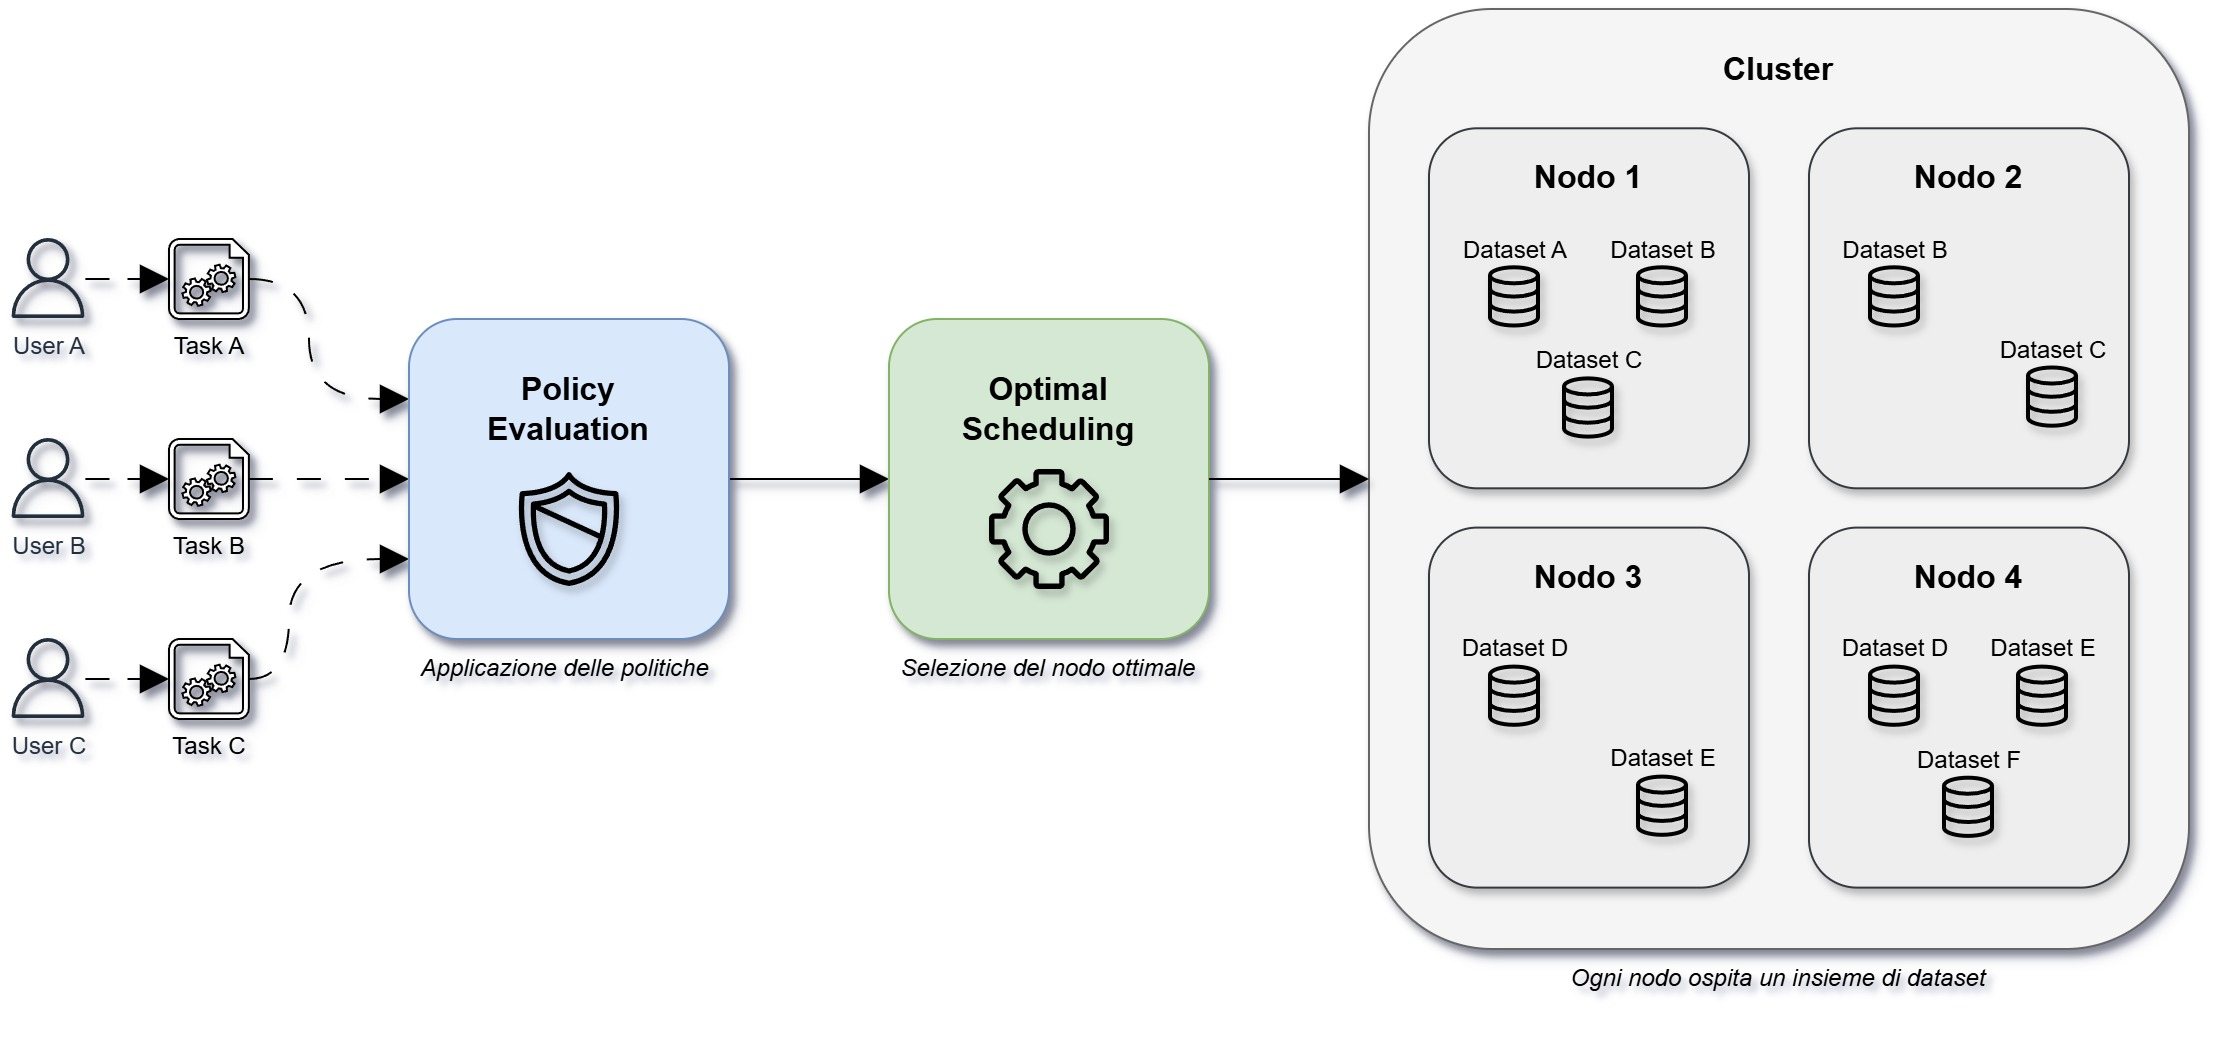
\includegraphics[width=\textwidth]{immagini/scenario.jpg}
    \caption{Architettura di riferimento del sistema.}
    \label{fig:scenario}
\end{figure}

L'aspetto più importante del problema riguarda la separazione delle responsabilità tra gli attori del sistema. Gli utenti esterni al sistema richiederanno l'esecuzione di task senza avere visibilità né controllo diretto sulla struttura interna del cluster o sulla distribuzione dei dataset: la loro interazione con il sistema si limita alla specifica dei requisiti del task. Invece, le politiche che governano la distribuzione sono definite a livello di sistema e hanno come obiettivo la protezione delle risorse rispetto agli utenti che le richiedono, garantendo che l'esecuzione avvenga soltanto in condizioni di compatibilità con il modello delle politiche.

Il problema affrontato in questa tesi consiste quindi nel progettare e realizzare un sistema \emph{policy-driven}, implementato in ambiente Kubernetes, in grado di ricevere richieste di esecuzione di task da parte di utenti esterni, valutarne i requisiti rispetto alle politiche associate alle risorse del cluster (definite secondo il modello che verrà introdotto nei capitoli successivi) e determinare, quando possibile, il nodo di esecuzione ottimale tra quelli che soddisfano tali vincoli. 

I lavori correlati che affrontano il problema dello scheduling \emph{policy-driven} in Kubernetes presentati in~\cite{policy-driven-sec-aware-scheduling-k8s, secure-k8s-workload-deployment} costituiscono un riferimento per il presente lavoro. Tuttavia, questa tesi si differenzia da tale approccio per l'introduzione esplicita di un modello formale dei vincoli tra le entità del sistema, seguendo un approccio simile a quanto già proposto in letteratura per la gestione e la classificazione delle risorse cloud in~\cite{sec-aware-data-alloc-multicloud, supp-sec-req-res-management-cloud, model-decision-data-storage-cloud}.

% ------------------------------------------------------------ %

\section{Assunzioni Preliminari}
\label{sec:assunzioni_preliminari}

Per descrivere il problema in modo più chiaro, è utile introdurre alcune assunzioni preliminari che ne delimitano il contesto e rendono il modello più gestibile. Queste assunzioni nascono dall'esigenza di mantenere il problema ben definito e affrontabile nell'ambito della tesi.

\paragraph{Distribuzione dei dataset}
\label{ass:dataset_distribuzione}

Ogni dataset è memorizzato localmente su uno o più nodi del cluster e, all'inizializzazione del sistema, si assume che la distribuzione iniziale dei dataset sia corretta, ovvero che non violi alcun vincolo associato ai dataset stessi. L'obiettivo del sistema non è quindi gestire la collocazione persistente dei dataset all'interno del cluster, ma valutare l'eventuale trasferimento logico o l'accesso remoto di un dataset verso il nodo selezionato per l'esecuzione di un task, nei casi in cui non sia già disponibile localmente su quel nodo. A tale operazione è associato un costo proporzionale alla dimensione del dataset, nota a priori, e la sua ammissibilità è subordinata al rispetto delle politiche di protezione associate al dataset. Questa scelta separa dunque il problema della collocazione persistente dei dataset, incluso lo spostamento fisico e la gestione della consistenza nel cluster, dal problema principale affrontato dal sistema, ovvero l'assegnazione dei task ai nodi e la valutazione del costo e dei vincoli dell'accesso remoto ai dati. In questo modo, il sistema integra costo e vincoli del trasferimento direttamente nel processo di selezione del nodo ottimale basandosi unicamente sui metadati necessari alla valutazione, senza dover realizzare un sottosistema dedicato allo spostamento fisico dei dati. Considerare anche il problema della distribuzione persistente dei dati introdurrebbe infatti una complessità aggiuntiva indipendente dagli obiettivi principali del lavoro. Il problema dell'allocazione fisica dei dati in un cluster o in ambiente cloud è comunque un aspetto ampiamente approfondito, ad esempio, nei lavori presentati in~\cite{sec-aware-data-alloc-multicloud, model-decision-data-storage-cloud}.

\paragraph{Visione globale del cluster}
\label{ass:visione_globale}

Al momento della sottomissione di un task da parte di un utente, il sistema dispone di una visione globale dello stato del cluster, che comprenderà sia le caratteristiche dei nodi sia la distribuzione corrente dei dataset su di essi. Questa assunzione è necessaria affinché il processo decisionale possa operare su informazioni complete e coerenti. Nel contesto di questa tesi tale aspetto è considerato risolto a livello infrastrutturale, in quanto Kubernetes espone nativamente un'interfaccia centralizzata per l'osservazione dello stato del cluster~\cite{k8s-comunication-nodes-control-plane, k8s-api}.

\paragraph{Esecuzione atomica dei task}
\label{ass:task_atomicita}

Ogni task viene eseguito interamente su un singolo nodo del cluster e non è prevista né la suddivisione di esso tra più nodi né la sua migrazione verso un nodo diverso dopo la sua assegnazione: la decisione di scheduling è quindi considerata definitiva al momento dell'assegnazione del task su un nodo. Questa ipotesi è coerente con il modello adottato da Kubernetes, che garantisce nativamente che ogni \texttt{Pod}, ossia la più piccola unità di lavoro che in questo contesto rappresenta il task, venga assegnato ed eseguito su un unico nodo, come descritto in~\cite{k8s-pods-atomic-node}.

\paragraph{Indipendenza dalla semantica dei task}
\label{ass:task_black_box}

Il sistema è indipendente dalla semantica interna dei task, che sono trattati come \emph{black-box} e considerati esclusivamente in termini delle loro proprietà, dei requisiti dichiarati e degli eventuali vincoli aggiuntivi rilevanti per il processo di assegnazione. Questa astrazione è necessaria per garantire la generalità del modello: un sistema dipendente dalla logica interna dei task risulterebbe infatti applicabile solo a domini di lavoro specifici, mentre l'obiettivo della tesi è definire un approccio di schedulazione generale indipendente dal tipo di operazioni che verranno eseguite.

\paragraph{Presenza di almeno un dataset richiesto}
\label{ass:dataset_minimo}

Ogni task richiede per la propria esecuzione almeno un dataset, coerentemente con il fatto che la computazione si fonda su di esso. Questa assunzione delimita il campo di applicazione del modello all'obiettivo della tesi, ovvero la distribuzione di task che utilizzano dataset soggetti a vincoli di protezione: un task privo di dataset richiesti non attiverebbe nessuna politica di protezione dei dati, ricadendo in un problema basilare di puro scheduling task-nodo.

% ------------------------------------------------------------ %

\section{Formalizzazione dei Concetti Base}
\label{sec:formalizzazione_base}

In questa sezione si introduce la formalizzazione del problema della tesi descritto nella Sezione~\ref{sec:scenario_applicativo}. L'obiettivo è rendere precisi i concetti di nodo, dataset, task e politica, e formulare il problema di assegnazione dei task in termini matematici. Le strutture introdotte in seguito saranno volutamente astratte e non approfondite: la loro descrizione concreta, ossia la definizione delle proprietà specifiche, dei vincoli delle entità e del contenuto delle politiche, è rimandata al Capitolo~\ref{cap:modello}.

% ------------------------------------------------------------ %

\subsection{Entità del Sistema e Distribuzione dei Dataset}
\label{subsec:entita_sistema}

Il sistema è definito da quattro insiemi fondamentali: l'insieme dei nodi $\mathcal{N}$, inteso come l'insieme dei nodi del cluster attivi e raggiungibili al momento della valutazione, l'insieme dei dataset disponibili nel sistema $\mathcal{D}$, l'insieme dei task $\mathcal{T}$ e l'insieme degli emittenti $\mathcal{I}$ (detti \emph{issuer}), che corrispondono ai soggetti che sottomettono i task nel sistema. A ogni task $t \in \mathcal{T}$ è associato il proprio emittente mediante la funzione:
\begin{equation}
    iss: \mathcal{T} \rightarrow \mathcal{I}
\end{equation}
tale che $iss(t)$ identifica l'issuer del task $t$. Inoltre, a ciascun task è associato l'insieme dei dataset necessari alla sua esecuzione, definito da:
\begin{equation}
    req: \mathcal{T} \rightarrow 2^\mathcal{D}
\end{equation}
ottenendo quindi $req(t) \subseteq \mathcal{D}$. Ad esempio, un task che per la sua esecuzione richiede due dataset $d_1$ e $d_2$ avrà $req(t) = \left\{ d_1,\, d_2 \right\}$.

Il primo elemento da formalizzare è la distribuzione dei dataset sui nodi del cluster. Poiché ogni dataset può essere disponibile su più nodi contemporaneamente, la collocazione dei dataset è definita dalla funzione descritta nella seguente Definizione~\ref{def:allocazione_dataset}. Un approccio simile è adottato in~\cite{sec-aware-data-alloc-multicloud}, dove la distribuzione di dati in scenari multicloud è modellata tenendo conto di requisiti di protezione associati a ciascuna risorsa.

\begin{definition}[Allocazione dei dataset]
    \label{def:allocazione_dataset}
    Lo stato di allocazione dei dataset nei nodi del cluster è definito dalla funzione:
    \begin{equation}
        \lambda: \mathcal{D} \rightarrow 2^\mathcal{N}
    \end{equation}
    dove $\lambda(d)$ indica l'insieme dei nodi in cui il dataset $d \in \mathcal{D}$ è disponibile localmente al momento della chiamata di funzione.
\end{definition}

Ad esempio, se attualmente i dataset $d_1$ e $d_2$ sono presenti localmente sui nodi $n_1$ e $n_2$, si avrà $\lambda(d_1) = \lambda(d_2) = \{n_1,\, n_2\}$. 
% La questione della dipendenza di $\lambda$ dal tempo, rilevante nei casi in cui l'allocazione evolve a seguito di trasferimenti tra nodi, sarà discussa nel Capitolo~\ref{cap:modello}, dove verrà chiarito in quale momento del processo di schedulazione lo stato di allocazione viene osservato dal sistema.

% ------------------------------------------------------------ %

\subsection{Famiglie di Politiche e Soddisfacibilità}
\label{subsec:famiglie_politiche}

Il cuore del sistema è costituito dall'insieme delle politiche, indicato con $\mathcal{C}$, che governano l'assegnazione dei task e l'eventuale trasferimento dei dati richiesti. Una politica esprime un vincolo che dovrà essere soddisfatto affinché un nodo possa essere considerato un candidato valido per l'esecuzione di un task. 

Le politiche in $\mathcal{C}$ operano a tre livelli distinti e coprono tre aspetti complementari del processo di assegnazione. Il primo sottoinsieme, denotato da $\mathcal{C_A} \subseteq \mathcal{C}$, raccoglie le politiche che determinano l'ammissibilità di un task $t$ nel sistema indipendentemente da qualunque nodo candidato: a differenza dei successivi sottoinsiemi, una politica in $\mathcal{C_A}$ non valuta la compatibilità tra il task e un nodo, ma stabilisce se il task possa essere preso in carico dal sistema solamente sulla base delle proprie proprietà, del proprio emittente, o dello stato corrente del sistema. Il secondo sottoinsieme, denotato da $\mathcal{C_T} \subseteq \mathcal{C}$, raccoglie le politiche che valutano la compatibilità diretta tra i requisiti del task $t$ e le caratteristiche del nodo candidato $n$: ad esempio, verificando che il nodo offra un certo livello di sicurezza o disponga delle risorse computazionali richieste. Il terzo sottoinsieme, denotato da $\mathcal{C_D} \subseteq \mathcal{C}$, regola invece il possibile trasferimento o accesso remoto dei dataset in $req(t)$ sul nodo candidato $n$: ad esempio, imponendo che il trasferimento di un dataset avvenga soltanto verso nodi situati in una determinata area geografica di riferimento, oppure che certi dataset non vengano trasferiti affatto.

I tre sottoinsiemi non sono necessariamente disgiunti tra loro: una politica che impone requisiti di sicurezza su un nodo può regolare contemporaneamente il trasferimento di dati verso di esso, appartenendo quindi sia a $\mathcal{C_T}$ sia a $\mathcal{C_D}$. Tuttavia, la loro unione copre l'intero insieme delle politiche:
\begin{equation}
    \mathcal{C} = \mathcal{C_A} \cup \mathcal{C_T} \cup \mathcal{C_D}
\end{equation}

Poiché le politiche operano su entità distinte, ovvero coppie nodo-task, coppie nodo-dataset e il task considerato indipendentemente da un nodo, si introduce una notazione di soddisfacibilità che copre tutti i casi. Per una politica $c \in \mathcal{C_T} \cup \mathcal{C_D}$, il vincolo riguarda la compatibilità tra un nodo candidato e il task o un dataset richiesto: scriviamo $n \models_t c$ per indicare che il nodo $n \in \mathcal{N}$ soddisfa la politica $c$ rispetto al task $t \in \mathcal{T}$, e $n \models_d c$ per indicare che il nodo $n$ soddisfa la politica $c$ rispetto al dataset $d \in \mathcal{D}$, ovvero che il possibile trasferimento di $d$ su $n$ è ammissibile secondo $c$. Invece, per una politica $c \in \mathcal{C_A}$ il vincolo riguarda esclusivamente il task, indipendentemente da qualunque nodo candidato: scriviamo $t \models c$ per indicare che il task $t \in \mathcal{T}$ soddisfa la politica $c$ rispetto al sistema, ovvero che $t$ è ammissibile nel sistema secondo $c$.

La stessa notazione si estende in modo naturale a un'intera famiglia di politiche, intendendo che ciascuna delle politiche che la compongono sia soddisfatta:
\begin{align}
    t \models \mathcal{C_A} &\iff \forall\, c \in \mathcal{C_A} :\; t \models c \\
    n \models_t \mathcal{C_T} &\iff \forall\, c \in \mathcal{C_T} :\; n \models_t c \\
    n \models_d \mathcal{C_D} &\iff \forall\, c \in \mathcal{C_D} :\; n \models_d c
\end{align}
Si tratta di semplici abbreviazioni, che verranno usate nel seguito quando non serve distinguere le singole politiche di una famiglia.

\begin{definition}[Soddisfacibilità delle politiche]
    \label{def:politiche}
    Sia $\mathcal{C}$ un insieme di politiche che il sistema deve rispettare durante la fase di assegnazione di un task. Ogni politica $c \in \mathcal{C}$ è un predicato che definisce un vincolo sul processo di assegnazione. La soddisfacibilità globale di tutte le politiche $\mathcal{C}$ rispetto a un task $t \in \mathcal{T}$ per un nodo candidato $n \in \mathcal{N}$ è definita come:
    \begin{equation}
        n \models_t \mathcal{C}
        \iff
        \left( \bigwedge_{c \in \mathcal{C_A}} t \models c \right)
        \land
        \left( \bigwedge_{c \in \mathcal{C_T}} n \models_t c \right)
        \land
        \left( \bigwedge_{\substack{c \in \mathcal{C_D}\\ d \in req(t)}} n \models_d c \right)
    \end{equation}
    Tale condizione equivale a richiedere $t \models \mathcal{C_A}$, $n \models_t \mathcal{C_T}$ e $n \models_d \mathcal{C_D}$ per ogni $d \in req(t)$.
\end{definition}

La condizione $n \models_t \mathcal{C}$ stabilisce quindi che il nodo $n$ può ammettere l'esecuzione del task $t$ se e solo se sono soddisfatte contemporaneamente tutte le condizioni definite dalle diverse famiglie di politiche discusse. In particolare, il task deve essere prima di tutto ammissibile nel sistema rispetto alle politiche indipendenti dal nodo $\mathcal{C_A}$, il nodo deve soddisfare i vincoli di compatibilità task-nodo definiti in $\mathcal{C_T}$, e, per ogni dataset $d \in req(t)$ richiesto, deve risultare ammissibile il suo possibile trasferimento o accesso remoto su $n$ secondo tutte le politiche nodo-dataset appartenenti a $\mathcal{C_D}$.

Da questa struttura, combinandola con l'assunzione di distribuzione iniziale corretta dei dataset, segue un risultato immediato riguardo i dataset già disponibili localmente su un nodo candidato.

\begin{theorem}[Correttezza dei dataset locali rispetto a $\mathcal{C_D}$]
    \label{teo:correttezza_locale}
    Per ogni dataset $d \in \mathcal{D}$ e per ogni nodo $n \in \mathcal{N}$, se $d$ è disponibile localmente su $n$, allora $n$ soddisfa tutte le politiche in $\mathcal{C_D}$ rispetto a $d$:
    \begin{equation}
        n \in \lambda(d) \implies n \models_d \mathcal{C_D}
        \qquad
        \forall\, d \in \mathcal{D},\, \forall\, n \in \mathcal{N}
    \end{equation}
    \begin{proof}
        Si dimostra per induzione sul numero $k$ di trasferimenti di dataset avvenuti nel sistema. 
        
        \paragraph{Caso base ($k = 0$)} All'inizializzazione del sistema, per assunzione, la distribuzione iniziale dei dataset è corretta: per ogni $d \in \mathcal{D}$ e ogni $n \in \lambda(d)$, vale $n \models_d \mathcal{C_D}$.
        
        \paragraph{Passo induttivo ($k > 0$)} Si supponga che la proprietà valga dopo $k$ trasferimenti, ovvero che per ogni $d \in \mathcal{D}$ e ogni $n \in \lambda(d)$ valga $n \models_d \mathcal{C_D}$. Sia ora $n' \notin \lambda(d')$ un nodo verso cui viene richiesto il $(k+1)$-esimo trasferimento di un dataset $d' \in \mathcal{D}$. Il trasferimento è ammesso dal sistema se e solo se $n' \models_{d'} \mathcal{C_D}$. Si distinguono ora due casi:
        \begin{itemize}
            \item  Se la condizione non è soddisfatta, il trasferimento viene rifiutato e $\lambda(d')$ rimane invariato. La proprietà continua a valere per ipotesi induttiva;
            \item Se la condizione è soddisfatta, il trasferimento viene eseguito e $\lambda(d')$ viene aggiornato con:
            \begin{equation}
                \lambda(d') \leftarrow \lambda(d') \cup \{n'\}
            \end{equation}
            Per i nodi già appartenenti a $\lambda(d')$ la proprietà continua a valere per ipotesi induttiva, mentre per $n'$ siamo nel caso in cui $n' \models_{d'} \mathcal{C_D}$ è soddisfatta. Di conseguenza, la validità della proprietà si estende al nuovo insieme $\lambda(d')$.
        \end{itemize}
        Dato che la proprietà è preservata in entrambi i casi, è dimostrato per induzione che:
        \begin{equation}
            n \in \lambda(d) \implies n \models_d \mathcal{C_D}
            \qquad 
            \forall d \in \mathcal{D}, \; \forall n \in \mathcal{N}
        \end{equation}
        è valida in ogni stato raggiungibile del sistema.
    \end{proof}
\end{theorem}

% ------------------------------------------------------------ %

\subsection{Nodi Ammissibili e Funzione di Ottimizzazione}
\label{subsec:nodi_ammissibili_score}

Ora, a partire dalla nozione di soddisfacibilità delle politiche, è possibile definire formalmente l'insieme dei nodi che sono candidati validi per l'esecuzione di un dato task rispetto ad un insieme di politiche di riferimento.

\begin{definition}[Nodi ammissibili]
    \label{def:nodi_ammissibili}
    Dato un task $t \in \mathcal{T}$ e un insieme di politiche $\mathcal{C}$, l'insieme dei nodi ammissibili (detti anche nodi candidati) per la sua assegnazione è definito come:
    \begin{equation}
        \mathcal{F_C}(t) = \left\{n \in \mathcal{N} \mid n \models_t \mathcal{C} \right\}
    \end{equation}
    ovvero l'insieme dei nodi che soddisfano tutte le politiche in $\mathcal{C}$ rispetto al task $t$.
\end{definition}

Con un leggero abuso di notazione, per una singola politica $c \in \mathcal{C}$ si scriverà $\mathcal{F}_c(t)$ al posto di $\mathcal{F}_{\{c\}}(t)$. Si noti che $\mathcal{F_C}(t)$ può essere vuoto per due motivi distinti. Il primo si verifica quando il task $t$ non risulta ammissibile rispetto a qualche politica in $\mathcal{C_A}$: in tal caso nessun nodo del cluster può soddisfare $n \models_t \mathcal{C}$, indipendentemente dalle caratteristiche dei nodi o dalla distribuzione dei dataset. Il secondo motivo si verifica invece quando, pur essendo $t$ ammissibile rispetto a $\mathcal{C_A}$, nessun nodo soddisfa contemporaneamente tutti i vincoli imposti dalle politiche in $\mathcal{C_T} \cup \mathcal{C_D}$.

Infine, tra i nodi ammissibili, il sistema dovrà selezionare quello ottimale. La qualità di un'assegnazione sarà quantificata da una funzione di ottimizzazione che combina un insieme di criteri di ottimizzazione, detti indicatori, seguendo un approccio simile a quello proposto in letteratura per la valutazione e classificazione di risorse sulla base di molteplici requisiti~\cite{cloud-plan-selection-req-multiple-app, supporting-user-requirement-pref-cloud}. La struttura della funzione riflette inoltre il modello di scoring adottato da Kubernetes, in cui ciascun plugin registrato nello scheduler contribuisce al punteggio complessivo con un peso configurabile~\cite{k8s-scheduler, k8s-scheduler-framework, k8s-scheduler-config}.

\begin{definition}[Funzione di ottimizzazione]
    \label{def:funzione_score}
    Sia $\Phi$ un insieme di indicatori, in cui ciascun $\phi \in \Phi$ è una funzione $\phi: \mathcal{N} \times \mathcal{T} \rightarrow [0,\, 1]$ che cattura un aspetto rilevante della qualità dell'assegnazione del task $t$ sul nodo $n$, e sia $w_\phi > 0$ il peso associato all'indicatore $\phi$. Dato un task $t \in \mathcal{T}$ e un insieme di politiche $\mathcal{C}$, per ogni nodo $n \in \mathcal{F_C}(t)$ la qualità dell'assegnazione è quantificata da una funzione di ottimizzazione definita come combinazione lineare pesata degli indicatori in $\Phi$:
    \begin{equation}
        \mathcal{S}_\Phi(n,\, t) = \sum_{\phi \in \Phi} w_\phi\, \phi(n,\, t)
    \end{equation}
\end{definition}

Come da definizione, ogni indicatore in $\Phi$ assume valori normalizzati nell'intervallo chiuso $[0,\, 1]$, al fine di garantire coerenza e uniformità tra le diverse metriche. Così come accade per le politiche in $\mathcal{C}$, il contenuto concreto dell'insieme $\Phi$ sarà definito nel successivo Capitolo~\ref{cap:modello}. 

% ------------------------------------------------------------ %

\subsection{Formulazione del Problema}
\label{subsec:formulazione_problema}

A questo punto, avendo introdotto tutti i concetti necessari alla descrizione del sistema, è possibile formulare in modo completo il problema di assegnazione.

\begin{problem}[Formulazione del problema]
    \label{def:formulazione_problema}
    Il problema consiste nel definire una funzione di assegnazione:
    \begin{equation}
        f: \mathcal{T} \rightarrow \mathcal{N} \cup \{\bot\}
    \end{equation}
    tale che, dati un task $t \in \mathcal{T}$, l'insieme globale delle politiche del sistema $\mathcal{C}$ e l'insieme degli indicatori $\Phi$, valga:
    \begin{equation}
        f(t) =
        \begin{cases}
            \arg\max_{n \in \mathcal{F_C}(t)}\, \mathcal{S}_\Phi(n,\, t)
                & \text{se } \mathcal{F_C}(t) \neq \emptyset \\
            \bot
                & \text{se } \mathcal{F_C}(t) = \emptyset
        \end{cases}
    \end{equation}
    Il caso in cui $f(t) = \bot$ indica che il task $t$ non potrà essere assegnato, in quanto nessun nodo del cluster soddisfa contemporaneamente tutte le politiche in $\mathcal{C}$ rispetto al task $t$:
    \begin{equation}
        f(t) = \bot \iff \nexists\, n \in \mathcal{N} :\; n \models_t \mathcal{C}
    \end{equation}
\end{problem}

Si osservi che il massimo di $\mathcal{S}_\Phi(n,\, t)$ su $\mathcal{F_C}(t)$ può essere raggiunto da più nodi. In tal caso, con $\arg\max$ si intende un qualunque elemento dell'insieme dei nodi di punteggio massimo, scelto secondo un criterio di spareggio arbitrario che il modello non vincola. 

Dunque, il processo di assegnazione di un task $t \in \mathcal{T}$ seguirà una pipeline composta dalle due fasi sequenziali di \emph{policy evaluation} e di \emph{optimal scheduling}, illustrata nella Figura~\ref{fig:flusso_schedulazione}. Il colore di ciascun riquadro indica la fase della pipeline a cui l'operazione appartiene: i riquadri grigi rappresentano passaggi non legati a una fase specifica; i riquadri blu corrispondono alla fase di \emph{policy evaluation}, dedicata alla valutazione delle politiche; i riquadri verdi corrispondono alla fase di \emph{optimal scheduling}, dedicata al calcolo della funzione di ottimizzazione sui nodi ammissibili; il riquadro rosso indica infine l'esito di rifiuto del task, $f(t) = \bot$. Questa convenzione cromatica viene mantenuta in tutte le figure analoghe presentate nei capitoli successivi.

\begin{figure}[htb]
    \centering
    \begin{tikzpicture}[
        node distance = 0.5cm,
        box/.style = {
            rectangle, rounded corners=3pt,
            minimum width=3cm, minimum height=1cm,
            text centered, draw=black, thick,
            font=\footnotesize, align=center
        },
        decision/.style = {
            diamond, aspect=2,
            minimum width=3cm, minimum height=1cm,
            text centered, draw=black, thick,
            font=\footnotesize, align=center
        },
        terminal/.style = {
            rectangle, rounded corners=6pt,
            minimum width=3cm, minimum height=1cm,
            text centered, draw=black, thick,
            font=\footnotesize, align=center
        },
        arrow/.style  = {-{Stealth[length=6pt]}, thick},
        label/.style  = {font=\scriptsize}
    ]
    
    \node[terminal, fill=gray!10] (task)
        {$t \in \mathcal{T}$};
    
    \node[decision, fill=dioblue, below=of task] (CA)
        {$t \models \mathcal{C_A}$};
    
    \node[box, fill=dioblue, below=of CA] (CT)
        {Valutazione $\mathcal{C_T}$\\
         \scriptsize $\forall\, n \in \mathcal{N}$};
    
    \node[box, fill=dioblue, below=of CT] (CD)
        {Valutazione $\mathcal{C_D}$\\
         \scriptsize $\forall\, d \in req(t),\, \forall\, n \in \mathcal{N}$};
    
    \node[decision, fill=gray!10, below=of CD] (dec)
        {$\mathcal{F_C}(t) \neq \emptyset$};
    
    \node[box, fill=diogreen, below=of dec] (score)
        {Calcolo $\mathcal{S}_\Phi(n,\,t)$\\[2pt]
         \scriptsize $\forall\, n \in \mathcal{F_C}(t)$};
    
    \node[terminal, fill=gray!10, below=of score] (ok)
        {$f(t) = \arg\max_{n \in \mathcal{F_C}(t)}\,\mathcal{S}_\Phi(n,\,t)$};
        
    \node[terminal, fill=diored, right=0.5cm of ok] (fail)
        {$f(t) = \bot$};
    
    \draw[arrow] (task)         -- (CA);
    \draw[arrow] (CA)           -- node[label, left]{sì} (CT);
    \draw[arrow] (CT)           -- (CD);
    \draw[arrow] (CD)           -- (dec);
    \draw[arrow] (dec)          -- node[label, left]{sì} (score);
    \draw[arrow] (score)        -- (ok);
    \draw[arrow] (CA.east)      -| node[label, above, near start]{no} (fail.north);
    \draw[arrow] (dec.east)     -| node[label, above, near start]{no} (fail.north);
    
    \end{tikzpicture}
    \caption{Pipeline di assegnazione di un task, articolata in una fase di filtraggio (riquadri blu) e una di ottimizzazione (riquadri verdi).}
    \label{fig:flusso_schedulazione}
\end{figure}

Dato l'insieme dei nodi del cluster $\mathcal{N}$, la pipeline esegue un filtraggio su tre livelli. Il primo livello verifica l'ammissibilità del task $t$ rispetto a $\mathcal{C_A}$, e nel caso in cui:
\begin{equation}
    \exists\, c \in \mathcal{C_A} :\; t \not\models c
\end{equation}
il task viene rifiutato immediatamente con $f(t) = \bot$, senza necessità di considerare alcun nodo del cluster. Superato questo primo livello, il sistema prosegue con il filtraggio dei nodi basato sulle politiche in $\mathcal{C_T} \cup \mathcal{C_D}$. Durante questo passaggio, un nodo $n$ viene escluso se vale:
\begin{equation} 
    \Bigl( \exists\, c \in \mathcal{C_T} :\; n \not\models_t c \Bigr) 
    \lor 
    \Bigl( \exists\, c \in \mathcal{C_D},\, \exists\, d \in req(t) :\; n \not\models_d c \Bigr) 
\end{equation}
Al termine di questa prima fase di filtraggio, l'insieme dei nodi ammissibili $\mathcal{F_C}(t)$ è completamente determinato: se risulta vuoto, il task non può essere assegnato e $f(t) = \bot$. Altrimenti, il sistema passa alla seconda fase di ottimizzazione in cui calcola $\mathcal{S}_\Phi(n,\, t)$ per ciascun $n \in \mathcal{F_C}(t)$ e seleziona il nodo con valore massimo come assegnazione finale $f(t)$.

% ------------------------------------------------------------ %

\section{Proprietà Desiderate del Sistema}
\label{sec:proprieta_desiderate}

A partire dalla definizione formale del problema, è possibile enunciare le principali garanzie che il modello soddisfa per costruzione. Si tratta di conseguenze dirette della funzione di assegnazione $f$, utili a chiarirne in modo rigoroso il comportamento e a servire come riferimento per la progettazione del sistema.

La prima e più fondamentale proprietà riguarda la correttezza dell'assegnazione: ogni volta che il sistema assegna un task a un nodo $n \in \mathcal{N}$, quell'assegnazione deve rispettare tutte le politiche definite in $\mathcal{C}$.

\begin{property}[Correttezza] 
    \label{prop:correttezza}
    Per ogni task $t \in \mathcal{T}$ tale che $f(t) \neq \bot$, il nodo assegnato deve soddisfare tutte le politiche in $\mathcal{C}$ rispetto al task $t$:
    \begin{equation}
        f(t) \neq \bot \implies f(t) \models_t \mathcal{C}
    \end{equation}
\end{property}

La funzione $f$ seleziona esclusivamente nodi in $\mathcal{F_C}(t)$, ovvero nodi che già soddisfano tutte le politiche in $\mathcal{C}$: non è quindi possibile che $f$ restituisca un nodo non ammissibile. La seconda proprietà riguarda la capacità del sistema di trovare sempre una soluzione quando essa esiste, definita come proprietà di completezza.

\begin{property}[Completezza] 
    \label{prop:completezza}
    Se esiste almeno un nodo ammissibile per il task $t$ per l'insieme di politiche $\mathcal{C}$ nel momento della sua sottomissione, il sistema è in grado di individuarlo e associarlo a $t$:
    \begin{equation}
        \mathcal{F_C}(t) \neq \emptyset \implies f(t) \neq \bot
    \end{equation}
\end{property}

Se $\mathcal{F_C}(t) \neq \emptyset$, la definizione di $f$ ne impone il calcolo dell'$\arg\max$ su tale insieme, che non può quindi restituire $\bot$. Viceversa, $f(t) = \bot$ si verifica soltanto quando $\mathcal{F_C}(t) = \emptyset$, ovvero quando nessun nodo soddisfa le politiche in $\mathcal{C}$. La terza proprietà riguarda la qualità della soluzione selezionata tra quelle ammissibili.

\begin{property}[Ottimalità] 
    \label{prop:ottimalita}
    Tra tutti i nodi ammissibili per il task $t$, il sistema seleziona quello con punteggio massimo rispetto alla funzione di ottimizzazione della Definizione~\ref{def:funzione_score}:
    \begin{equation}
        f(t) \neq \bot \implies f(t) = \arg\max_{n \in \mathcal{F_C}(t)}\,\mathcal{S}_\Phi(n,\,t)
    \end{equation}
\end{property}

Anche in questo caso, l'$\arg\max$ della definizione di $f$ seleziona per costruzione il nodo di punteggio massimo tra quelli ammissibili quando esistono.

Inoltre, la minimizzazione del trasferimento di dati remoti è una conseguenza diretta della Proprietà~\ref{prop:ottimalita} nel momento in cui il costo di trasferimento è catturato da uno o più indicatori in $\Phi$ che crescono al diminuire del volume di dati remoti. Perciò, stando alla struttura della funzione di ottimizzazione, a parità di punteggio rispetto a tutti gli altri criteri di ottimizzazione, il sistema privilegia i nodi che minimizzano il trasferimento o l'accesso a dataset remoti.